
\documentclass[12pt]{article}
\usepackage[brazil]{babel} % para relatórios em português
\usepackage[utf8]{inputenc} % para acentuação direta
\usepackage{amsmath,amsfonts,amssymb}  % improve math presentation
\usepackage{tabularx} % extra features for tabular environment
\usepackage{graphicx} % takes care of graphic including machinery
\usepackage[margin=0.8in,letterpaper]{geometry} % decreases margins
\usepackage[final]{hyperref} % adds hyper links inside the generated pdf file
\usepackage{xcolor}
%\usepackage[pdftex]{hyperref}

\hypersetup{
	colorlinks=true,       % false: boxed links; true: colored links
	linkcolor=blue,        % color of internal links
	citecolor=blue,        % color of links to bibliography
	filecolor=magenta,     % color of file links
	urlcolor=blue
}

\begin{document}

\title{Manual para usar o HigFlow no cluster Euler}
\author{HigFlow e HigTree}
\date{\today}
\maketitle

\section{Cluster - Passos iniciais}\label{sec:clu_pas_ini}

Para que consiga utilizar o cluster para realizar os testes do HigFlow, inicialmente deve-se criar uma conta pelo do site \href{http://www.cemeai.icmc.usp.br/Euler/index.html}{site do Cluster}( Manual para uso do cluster - \href{http://resources.altair.com/pbs/documentation/support/PBSProUserGuide12.2.pdf}{manual}). Para enviar o código para cluster, deve inicialmente criar uma pasta no cluster onde será armazenado o código. Para o envio existem duas possibilidades
\begin{itemize}
	\item \textbf{git clone https://github.com/antoniocastelofilho/HigFlow.git} $:=$ faz uma cópia do código armazenado no GitHub. Para esse caso, deve-se ter acesso ao projeto no GitHub
	\item \textbf{scp -r diretorio usuario@euler.cemeai.icmc.usp.br:/diretorio\_de\_destino\_no\_cluster/}	$:=$ Envia o ``diretorio" (com o código do HigFlow) para o cluster Euler para o ``diretorio\_de\_destino\_no\_cluster"
\end{itemize}
 
 Após o envio do código, deve-se alterar o arquivo ``bashrc" do cluster seguindo os passos abaixo:
 \begin{itemize}
 	\item \textbf{vi $\sim$/.bashrc} $:=$ Abre o arquivo ``bashrc" para ser editado pelo \textbf{vi};
 	\item Acrescente as linhas a seguir no arquivo ``bashrc":\\
 	\textbf{export HIGTREE\_DIR=/diretorio\_do\_higflow\_no\_cluster/higtree}\\
 	\textbf{export HIGFLOW\_DIR=/diretorio\_do\_higflow\_no\_cluster/higflow}\\
 	
 	\textbf{Exemplo:} Como exemplo, no usuário ``juniormr" fez-se o download do código no diretório ``/lustre/juniormr/HigFlow", assim as linhas adicionadas serão\\
 	\begin{figure}[htb]
 		\centering
 		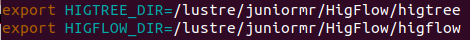
\includegraphics[width=0.98\linewidth]{figures/export_bashrc}
 		\label{fig:fig01}
 	\end{figure}
 \end{itemize}

\section{Modulo ``higtree/deps" para o sistema HigFlow no cluster}

Para conseguir compilar o código no cluster é necessário carregar o modulo ``higtree/deps", fazendo
\begin{itemize}
	\item \textbf{module load higtree/deps} $:=$ Comando que carrega os módulos necessários para compilar;
	\item \textbf{module list} $:=$ Comando para mostrar os módulos carregados. Quando carregado o modulo ``higtree/deps", ao digitar ``module list" tem-se
	\begin{figure}[htb]
		\centering
		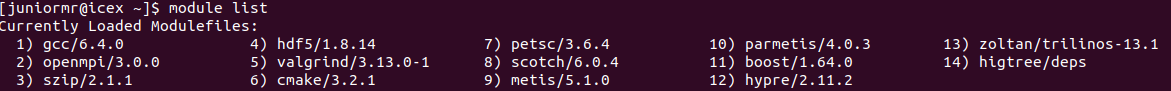
\includegraphics[width=1.0\linewidth]{figures/module_list}
		\label{fig:fig02}
	\end{figure}
\end{itemize}

\section{Job}\label{sec:job_fun}

Para rodar os teste é necessário criar um arquivo ``.job" para submeter ao cluster. Abaixo segue um exemplo
\begin{figure}[htb]
	\centering
	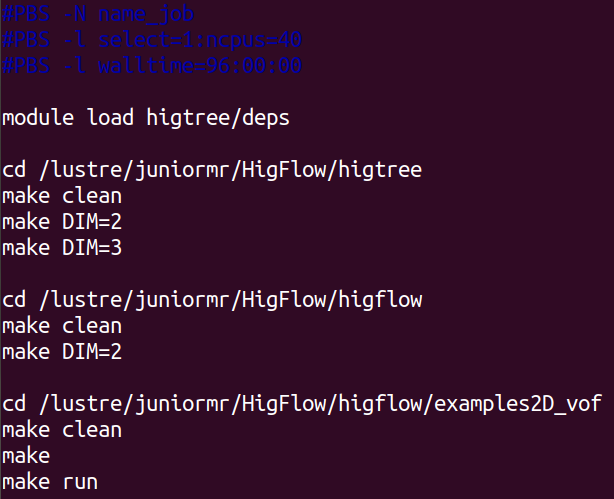
\includegraphics[width=0.80\linewidth]{figures/submission_job}
	\label{fig:fig03}
\end{figure}


%\bibliographystyle{plain}
%\bibliography{cluster_euler}

\end{document}
